\chapter{Dataset Background}
The dataset used in the prototype applications is a real world dataset taken from the biological environment. The data is constructed by an ontology derived from the combined research projects undertaken on the e-Mouse Atlas Project (EMAP) by Dr Duncan Davidson and Professor Richard Baldock.\begin{wrapfigure}{r}{0.25\textwidth}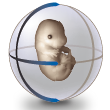
\includegraphics[width=0.9\linewidth]{images/ema_logo}\end{wrapfigure} The name EMAP carries a certain amount of ambiguity as it is the name of the project that developed the anatomy, and is also the name of the anatomy itself. Therefore with the motivation of clarity, I will refer to the project that developed the anatomy as e-Mouse Atlas (EMA) and the name of the anatomy as EMAP. Inspired by the findings of Theiler (1989) and Kaufman (1992), EMA uses embryological mouse models to provide a detailed map of mouse development. The EMAP has a developed collection of three dimensional computer models of mouse embryos at the consecutive stages of growth generation with anatomical domains joined by an ontology of anatomical names. The main deliverable of the EMA resource is to provide a comprehensive visualisation of the post-implantation of mouse development and to induct an investigation of the gene expression in the post-implantation mouse embryo.

\section{Discussion}
The EMA ontology has several different branch deliverables, each provides an alternative aspect of the evolution of a mouse embryo. The branches which will be utilised for this research project are the timed stage specific structure, EMAP and the aggregated non stage specific e-mouse Atlas Project Abstract (EMAPA) which are respectively discussed below [REFERENCE]. The EMA dataset's were chosen as the source of data for this research as it is a freely available, rich and substantial data source.

\subsection{EMAP}
The devised EMAP ontology was originally developed to deliver a structured and controlled vocabulary of stage-specific anatomical structures for the developing laboratory mouse. As the EMA research has progressed, the ontology has followed suit, and is continually under development. The current ontology is in scope for a forthcoming release.
Based on the timed component stage-specific Theiler development of a mouse embryo, the EMAP dataset combined the stage identifier and the anatomical name based on the researched information for the respective development stage. The timed components are regarded as the main aspect of the ontology and the abstract, non-stage-specific terms came as a secondary protocol.

A hierarchical structure for each of the Theiler stages has been developed and are presented in separate directed acyclic graphs. This data is available in an obo-formatted file; which I will discuss later in the document. [REFERENCE]

The intended outcome of this version of the EMAP was to provide information about the shape, gross anatomy and detailed histological structure of the mouse.

\subsection{EMAPA}
The EMAPA structure is a refined and developed non-stage specific representation of the mouse anatomy ontology. This enhanced version of the ontology is now considered as the primary EMA anatomy ontology and will form the basis of the dataset for this research. As with the EMAP structure the EMAPA is available in 

\section{Data Sources}
\subsection{EMA Database}
\subsection{OBO}
\subsection{OWL}
